% Options for packages loaded elsewhere
\PassOptionsToPackage{unicode}{hyperref}
\PassOptionsToPackage{hyphens}{url}
%
\documentclass[
]{article}
\usepackage{lmodern}
\usepackage{amsmath}
\usepackage{ifxetex,ifluatex}
\ifnum 0\ifxetex 1\fi\ifluatex 1\fi=0 % if pdftex
  \usepackage[T1]{fontenc}
  \usepackage[utf8]{inputenc}
  \usepackage{textcomp} % provide euro and other symbols
  \usepackage{amssymb}
\else % if luatex or xetex
  \usepackage{unicode-math}
  \defaultfontfeatures{Scale=MatchLowercase}
  \defaultfontfeatures[\rmfamily]{Ligatures=TeX,Scale=1}
\fi
% Use upquote if available, for straight quotes in verbatim environments
\IfFileExists{upquote.sty}{\usepackage{upquote}}{}
\IfFileExists{microtype.sty}{% use microtype if available
  \usepackage[]{microtype}
  \UseMicrotypeSet[protrusion]{basicmath} % disable protrusion for tt fonts
}{}
\makeatletter
\@ifundefined{KOMAClassName}{% if non-KOMA class
  \IfFileExists{parskip.sty}{%
    \usepackage{parskip}
  }{% else
    \setlength{\parindent}{0pt}
    \setlength{\parskip}{6pt plus 2pt minus 1pt}}
}{% if KOMA class
  \KOMAoptions{parskip=half}}
\makeatother
\usepackage{xcolor}
\IfFileExists{xurl.sty}{\usepackage{xurl}}{} % add URL line breaks if available
\IfFileExists{bookmark.sty}{\usepackage{bookmark}}{\usepackage{hyperref}}
\hypersetup{
  pdftitle={Cheating Charts : JTBC 20150303},
  pdfauthor={coop711},
  hidelinks,
  pdfcreator={LaTeX via pandoc}}
\urlstyle{same} % disable monospaced font for URLs
\usepackage[margin=1in]{geometry}
\usepackage{color}
\usepackage{fancyvrb}
\newcommand{\VerbBar}{|}
\newcommand{\VERB}{\Verb[commandchars=\\\{\}]}
\DefineVerbatimEnvironment{Highlighting}{Verbatim}{commandchars=\\\{\}}
% Add ',fontsize=\small' for more characters per line
\usepackage{framed}
\definecolor{shadecolor}{RGB}{248,248,248}
\newenvironment{Shaded}{\begin{snugshade}}{\end{snugshade}}
\newcommand{\AlertTok}[1]{\textcolor[rgb]{0.94,0.16,0.16}{#1}}
\newcommand{\AnnotationTok}[1]{\textcolor[rgb]{0.56,0.35,0.01}{\textbf{\textit{#1}}}}
\newcommand{\AttributeTok}[1]{\textcolor[rgb]{0.77,0.63,0.00}{#1}}
\newcommand{\BaseNTok}[1]{\textcolor[rgb]{0.00,0.00,0.81}{#1}}
\newcommand{\BuiltInTok}[1]{#1}
\newcommand{\CharTok}[1]{\textcolor[rgb]{0.31,0.60,0.02}{#1}}
\newcommand{\CommentTok}[1]{\textcolor[rgb]{0.56,0.35,0.01}{\textit{#1}}}
\newcommand{\CommentVarTok}[1]{\textcolor[rgb]{0.56,0.35,0.01}{\textbf{\textit{#1}}}}
\newcommand{\ConstantTok}[1]{\textcolor[rgb]{0.00,0.00,0.00}{#1}}
\newcommand{\ControlFlowTok}[1]{\textcolor[rgb]{0.13,0.29,0.53}{\textbf{#1}}}
\newcommand{\DataTypeTok}[1]{\textcolor[rgb]{0.13,0.29,0.53}{#1}}
\newcommand{\DecValTok}[1]{\textcolor[rgb]{0.00,0.00,0.81}{#1}}
\newcommand{\DocumentationTok}[1]{\textcolor[rgb]{0.56,0.35,0.01}{\textbf{\textit{#1}}}}
\newcommand{\ErrorTok}[1]{\textcolor[rgb]{0.64,0.00,0.00}{\textbf{#1}}}
\newcommand{\ExtensionTok}[1]{#1}
\newcommand{\FloatTok}[1]{\textcolor[rgb]{0.00,0.00,0.81}{#1}}
\newcommand{\FunctionTok}[1]{\textcolor[rgb]{0.00,0.00,0.00}{#1}}
\newcommand{\ImportTok}[1]{#1}
\newcommand{\InformationTok}[1]{\textcolor[rgb]{0.56,0.35,0.01}{\textbf{\textit{#1}}}}
\newcommand{\KeywordTok}[1]{\textcolor[rgb]{0.13,0.29,0.53}{\textbf{#1}}}
\newcommand{\NormalTok}[1]{#1}
\newcommand{\OperatorTok}[1]{\textcolor[rgb]{0.81,0.36,0.00}{\textbf{#1}}}
\newcommand{\OtherTok}[1]{\textcolor[rgb]{0.56,0.35,0.01}{#1}}
\newcommand{\PreprocessorTok}[1]{\textcolor[rgb]{0.56,0.35,0.01}{\textit{#1}}}
\newcommand{\RegionMarkerTok}[1]{#1}
\newcommand{\SpecialCharTok}[1]{\textcolor[rgb]{0.00,0.00,0.00}{#1}}
\newcommand{\SpecialStringTok}[1]{\textcolor[rgb]{0.31,0.60,0.02}{#1}}
\newcommand{\StringTok}[1]{\textcolor[rgb]{0.31,0.60,0.02}{#1}}
\newcommand{\VariableTok}[1]{\textcolor[rgb]{0.00,0.00,0.00}{#1}}
\newcommand{\VerbatimStringTok}[1]{\textcolor[rgb]{0.31,0.60,0.02}{#1}}
\newcommand{\WarningTok}[1]{\textcolor[rgb]{0.56,0.35,0.01}{\textbf{\textit{#1}}}}
\usepackage{longtable,booktabs}
\usepackage{calc} % for calculating minipage widths
% Correct order of tables after \paragraph or \subparagraph
\usepackage{etoolbox}
\makeatletter
\patchcmd\longtable{\par}{\if@noskipsec\mbox{}\fi\par}{}{}
\makeatother
% Allow footnotes in longtable head/foot
\IfFileExists{footnotehyper.sty}{\usepackage{footnotehyper}}{\usepackage{footnote}}
\makesavenoteenv{longtable}
\usepackage{graphicx}
\makeatletter
\def\maxwidth{\ifdim\Gin@nat@width>\linewidth\linewidth\else\Gin@nat@width\fi}
\def\maxheight{\ifdim\Gin@nat@height>\textheight\textheight\else\Gin@nat@height\fi}
\makeatother
% Scale images if necessary, so that they will not overflow the page
% margins by default, and it is still possible to overwrite the defaults
% using explicit options in \includegraphics[width, height, ...]{}
\setkeys{Gin}{width=\maxwidth,height=\maxheight,keepaspectratio}
% Set default figure placement to htbp
\makeatletter
\def\fps@figure{htbp}
\makeatother
\setlength{\emergencystretch}{3em} % prevent overfull lines
\providecommand{\tightlist}{%
  \setlength{\itemsep}{0pt}\setlength{\parskip}{0pt}}
\setcounter{secnumdepth}{-\maxdimen} % remove section numbering
\ifluatex
  \usepackage{selnolig}  % disable illegal ligatures
\fi

\title{Cheating Charts : JTBC 20150303}
\author{coop711}
\date{2021-02-17}

\begin{document}
\maketitle

\hypertarget{problem}{%
\section{Problem,}\label{problem}}

JTBC 뉴스룸에서 김영란법 국회 통과에 관련하여 여론조사한 결과라고 보여
준 자료는 더 이상 남아 있지 않으나 트위터에 다음과 같은 내용으로 남아
있다. 어딘가 이상하다.

\begin{Shaded}
\begin{Highlighting}[]
\FunctionTok{include\_graphics}\NormalTok{(}\StringTok{"../pics/JTBC\_20150303.png"}\NormalTok{)}
\end{Highlighting}
\end{Shaded}

\begin{center}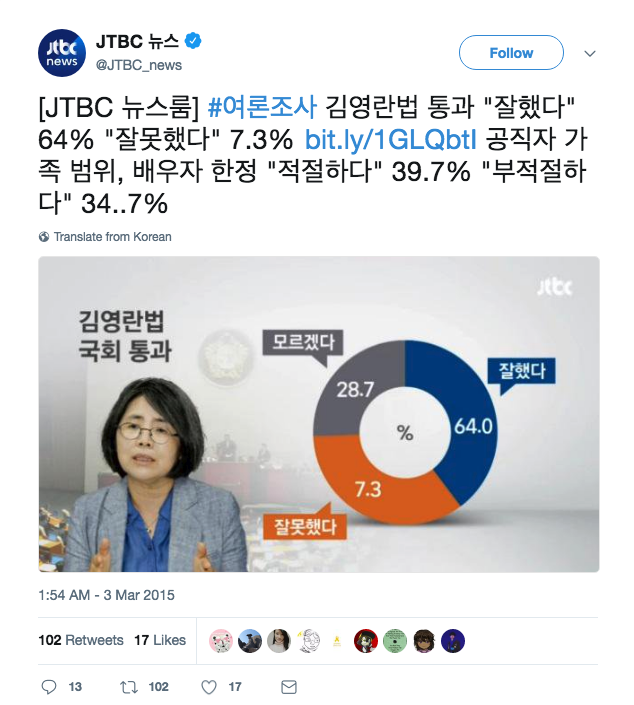
\includegraphics[width=0.5\linewidth]{../pics/JTBC_20150303} \end{center}

이 도표의 문제점을 여러 네티즌들이 지적하였더니 방송본에는 다음과 같은
스크린캡처가 남아 있다.

\begin{Shaded}
\begin{Highlighting}[]
\FunctionTok{include\_graphics}\NormalTok{(}\StringTok{"../pics/JTBC\_20150303v2.png"}\NormalTok{)}
\end{Highlighting}
\end{Shaded}

\begin{center}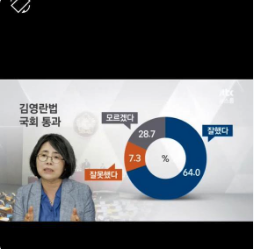
\includegraphics[width=0.45\linewidth]{../pics/JTBC_20150303v2} \end{center}

이 도표를 제대로 그려보자.

\hypertarget{math}{%
\section{Math}\label{math}}

Base R의 \texttt{pie()}함수를 활용한다. 도표 안의 텍스트 라벨 좌표는
극좌표 변환식 \(x = r \cos(\theta),\; y = r \sin(\theta)\)를 이용한다.

각 텍스트 라벨의 좌표를 계산하려면 64.0의 각도가 0으로 세팅되어 있음에
유의하고, 극좌표의 각도를 계산하기 위하여 시계 반대 방향으로 90도가
25\%에 해당한다는 점에 착안한다. 텍스트 라벨 7.3이 새겨져 있는 각도가
28.7\%와 7.3\%의 가운데이므로 (25\% + 28.7\%)와 (25\% + 28.7\% +
7.3\%)의 가운데이고 이를 각도로 표현하면
\(\frac{(25 + 28.7) + (25 + 28.7 + 7.3)}{2}\times\frac{1}{100}\times2\pi\)이
된다. 같은 방식으로 텍스트 라벨 28.7이 새겨진 위치의 각도는 25\%와 (25\%
+ 28.7\%)의 가운데인
\(\frac{25 + (25 + 28.7)}{2}\times\frac{1}{100}\times2\pi\) 이 된다.

또는 텍스트 라벨 7.3의 위치를 25\% + 27.8\% 에서 7.3\%의 반을 더한
것으로 이해하여도 된다. 이 때의 식은
\((25 + 28.7 + 7.3/2)\times\frac{1}{100}\times2\pi\)으로 표현할 수 있다.
텍스트 라벨 28.7의 위치는 25\%에서 28.7\%의 반을 더한 위치,
\((25 + 28.7/2)\times\frac{1}{100}\times2\pi\)이 된다.

\hypertarget{programming}{%
\section{Programming}\label{programming}}

\hypertarget{data}{%
\subsection{Data}\label{data}}

\begin{Shaded}
\begin{Highlighting}[]
\NormalTok{poll }\OtherTok{\textless{}{-}} \FunctionTok{c}\NormalTok{(}\FloatTok{64.0}\NormalTok{, }\FloatTok{7.3}\NormalTok{, }\FloatTok{28.7}\NormalTok{)}
\FunctionTok{names}\NormalTok{(poll) }\OtherTok{\textless{}{-}} \FunctionTok{c}\NormalTok{(}\StringTok{"잘했다"}\NormalTok{, }\StringTok{"잘못했다"}\NormalTok{, }\StringTok{"모르겠다"}\NormalTok{)}
\CommentTok{\#\textgreater{} 도표 안 레이블의 좌표 계산. 각도를 어떻게 계산하는지 유의할 것}
\NormalTok{pos }\OtherTok{\textless{}{-}} \FunctionTok{cumsum}\NormalTok{(poll) }\SpecialCharTok{{-}}\NormalTok{ poll }\SpecialCharTok{/} \DecValTok{2}
\NormalTok{x\_text }\OtherTok{\textless{}{-}} \FloatTok{0.75} \SpecialCharTok{*} \FunctionTok{cos}\NormalTok{(pi }\SpecialCharTok{/} \DecValTok{2} \SpecialCharTok{{-}}\NormalTok{ (}\DecValTok{2} \SpecialCharTok{*}\NormalTok{ pi) }\SpecialCharTok{*}\NormalTok{ pos }\SpecialCharTok{/} \DecValTok{100}\NormalTok{)}
\NormalTok{y\_text }\OtherTok{\textless{}{-}} \FloatTok{0.75} \SpecialCharTok{*} \FunctionTok{sin}\NormalTok{(pi }\SpecialCharTok{/} \DecValTok{2} \SpecialCharTok{{-}}\NormalTok{ (}\DecValTok{2} \SpecialCharTok{*}\NormalTok{ pi) }\SpecialCharTok{*}\NormalTok{ pos }\SpecialCharTok{/} \DecValTok{100}\NormalTok{)}
\CommentTok{\# x\_text \textless{}{-} 0.75 * cos(c(0, }
\CommentTok{\#                        ((25 + 28.7) + (25 + 28.7 + 7.3)) * pi / 100, }
\CommentTok{\#                        (25 + (25 + 28.7)) * pi / 100))}
\CommentTok{\# y\_text \textless{}{-} 0.75 * sin(c(0, }
\CommentTok{\#                        ((25 + 28.7) + (25 + 28.7 + 7.3)) * pi / 100, }
\CommentTok{\#                        (25 + (25 + 28.7)) * pi / 100))}
\NormalTok{x\_text0 }\OtherTok{\textless{}{-}}\NormalTok{ x\_text}
\NormalTok{y\_text0 }\OtherTok{\textless{}{-}}\NormalTok{ y\_text}
\NormalTok{x\_text[}\DecValTok{1}\NormalTok{] }\OtherTok{\textless{}{-}} \FloatTok{0.75}
\NormalTok{y\_text[}\DecValTok{1}\NormalTok{] }\OtherTok{\textless{}{-}} \DecValTok{0}
\FunctionTok{kable}\NormalTok{(}\FunctionTok{t}\NormalTok{(}\FunctionTok{as.matrix}\NormalTok{(poll)), }\AttributeTok{caption =} \StringTok{"김영란법 국회 통과"}\NormalTok{)}
\end{Highlighting}
\end{Shaded}

\begin{longtable}[]{@{}rrr@{}}
\caption{김영란법 국회 통과}\tabularnewline
\toprule
잘했다 & 잘못했다 & 모르겠다\tabularnewline
\midrule
\endfirsthead
\toprule
잘했다 & 잘못했다 & 모르겠다\tabularnewline
\midrule
\endhead
64 & 7.3 & 28.7\tabularnewline
\bottomrule
\end{longtable}

\hypertarget{pie}{%
\subsection{\texorpdfstring{\texttt{pie()}}{pie()}}\label{pie}}

\begin{Shaded}
\begin{Highlighting}[]
\CommentTok{\# font\_add(family = "NanumGothic", regular = "NanumFont/NanumGothic.ttf")}
\FunctionTok{showtext\_auto}\NormalTok{()}
\CommentTok{\# par(family = "NanumGothic")}
\FunctionTok{font\_add}\NormalTok{(}\AttributeTok{family =} \StringTok{"KoPubWorld Dotum Medium"}\NormalTok{, }\AttributeTok{regular =} \StringTok{"KoPubWorld/KoPubWorld Dotum Medium.ttf"}\NormalTok{)}
\FunctionTok{font\_add}\NormalTok{(}\AttributeTok{family =} \StringTok{"KoPubWorld Dotum Bold"}\NormalTok{, }\AttributeTok{regular =} \StringTok{"KoPubWorld/KoPubWorld Dotum Bold.ttf"}\NormalTok{)}
\CommentTok{\# showtext\_auto()}
\FunctionTok{par}\NormalTok{(}\AttributeTok{family =} \StringTok{"KoPubWorld Dotum Medium"}\NormalTok{)}
\FunctionTok{pie}\NormalTok{(poll, }
    \AttributeTok{labels =} \StringTok{""}\NormalTok{, }
    \AttributeTok{radius =} \DecValTok{1}\NormalTok{,}
    \AttributeTok{clockwise =} \ConstantTok{TRUE}\NormalTok{, }
    \AttributeTok{init.angle =} \DecValTok{90}\NormalTok{, }
    \AttributeTok{cex =} \FloatTok{1.5}\NormalTok{,}
    \AttributeTok{col =} \FunctionTok{c}\NormalTok{(}\StringTok{"blue"}\NormalTok{, }\StringTok{"red"}\NormalTok{, }\StringTok{"grey"}\NormalTok{))}
\FunctionTok{par}\NormalTok{(}\AttributeTok{new =} \ConstantTok{TRUE}\NormalTok{)}
\FunctionTok{pie}\NormalTok{(}\DecValTok{1}\NormalTok{,}
    \AttributeTok{labels =} \StringTok{""}\NormalTok{,}
    \AttributeTok{radius =} \FloatTok{0.5}\NormalTok{,}
    \AttributeTok{border =} \ConstantTok{NA}\NormalTok{,}
    \AttributeTok{col =} \StringTok{"white"}\NormalTok{)}
\FunctionTok{text}\NormalTok{(}\AttributeTok{x =} \DecValTok{0}\NormalTok{, }\AttributeTok{y =} \DecValTok{0}\NormalTok{, }
     \AttributeTok{labels =} \StringTok{"\%"}\NormalTok{, }
     \AttributeTok{cex =} \FloatTok{1.5}\NormalTok{)}
\FunctionTok{text}\NormalTok{(}\AttributeTok{x =}\NormalTok{ x\_text, }\AttributeTok{y =}\NormalTok{ y\_text, }
     \AttributeTok{labels =} \FunctionTok{format}\NormalTok{(poll, }\AttributeTok{nsmall =} \DecValTok{1}\NormalTok{), }
     \AttributeTok{col =} \StringTok{"white"}\NormalTok{, }
     \AttributeTok{cex =} \FloatTok{1.5}\NormalTok{)}
\FunctionTok{rect}\NormalTok{(}\FloatTok{2.1} \SpecialCharTok{*}\NormalTok{ x\_text0 }\SpecialCharTok{{-}} \FloatTok{0.6}\NormalTok{, }\FloatTok{2.1} \SpecialCharTok{*}\NormalTok{ y\_text0 }\SpecialCharTok{{-}} \FloatTok{0.1}\NormalTok{, }
     \FloatTok{2.1} \SpecialCharTok{*}\NormalTok{ x\_text0 }\SpecialCharTok{+} \FloatTok{0.6}\NormalTok{, }\FloatTok{2.1} \SpecialCharTok{*}\NormalTok{ y\_text0 }\SpecialCharTok{+} \FloatTok{0.1}\NormalTok{,}
     \AttributeTok{col =} \FunctionTok{c}\NormalTok{(}\StringTok{"blue"}\NormalTok{, }\StringTok{"red"}\NormalTok{, }\StringTok{"grey"}\NormalTok{),}
     \AttributeTok{border =} \StringTok{"black"}\NormalTok{)}
\FunctionTok{text}\NormalTok{(}\AttributeTok{x =} \FloatTok{2.1} \SpecialCharTok{*}\NormalTok{ x\_text0, }\AttributeTok{y =} \FloatTok{2.1} \SpecialCharTok{*}\NormalTok{ y\_text0, }
     \AttributeTok{labels =} \FunctionTok{names}\NormalTok{(poll), }
     \AttributeTok{col =} \StringTok{"white"}\NormalTok{, }
     \AttributeTok{cex =} \FloatTok{1.5}\NormalTok{)}
\FunctionTok{title}\NormalTok{(}\AttributeTok{main =} \StringTok{"김영란법}\SpecialCharTok{\textbackslash{}n}\StringTok{국회 통과"}\NormalTok{, }\AttributeTok{cex.main =} \DecValTok{2}\NormalTok{, }\AttributeTok{family =} \StringTok{"KoPubWorld Dotum Bold"}\NormalTok{)}
\FunctionTok{box}\NormalTok{(}\AttributeTok{which =} \StringTok{"figure"}\NormalTok{, }\AttributeTok{lwd =} \DecValTok{3}\NormalTok{)}
\end{Highlighting}
\end{Shaded}

\begin{center}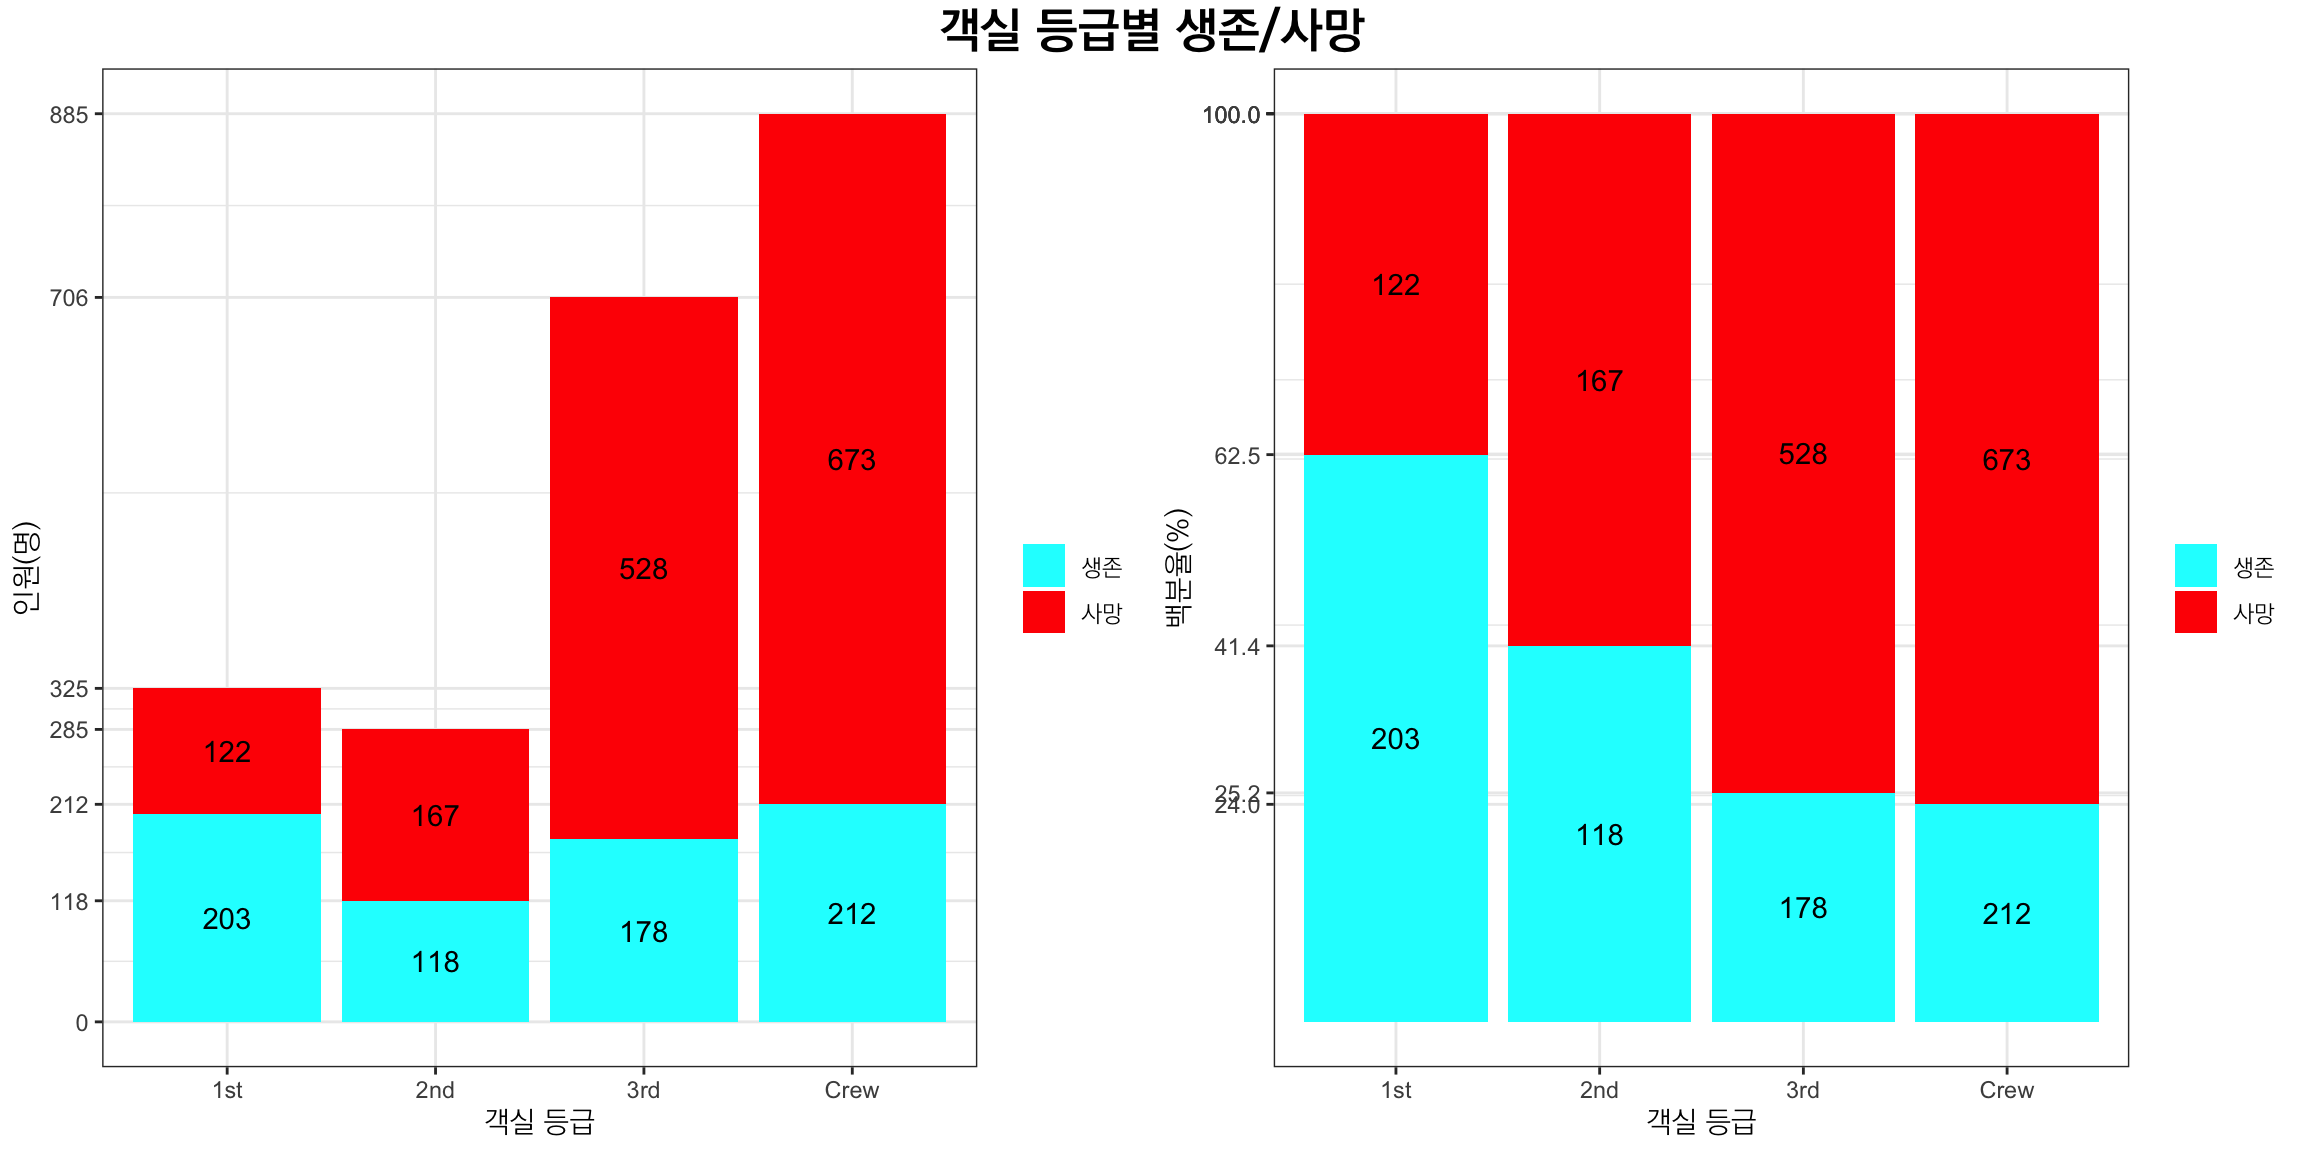
\includegraphics[width=0.67\linewidth]{JTBC_20150303_ggplot_v2_files/figure-latex/unnamed-chunk-4-1} \end{center}

\begin{Shaded}
\begin{Highlighting}[]
\FunctionTok{dev.copy}\NormalTok{(png, }\StringTok{"../pics/jtbc150303.png"}\NormalTok{, }\AttributeTok{width =} \DecValTok{480}\NormalTok{, }\AttributeTok{height =} \DecValTok{480}\NormalTok{)}
\end{Highlighting}
\end{Shaded}

\begin{verbatim}
## png 
##   3
\end{verbatim}

\begin{Shaded}
\begin{Highlighting}[]
\FunctionTok{dev.off}\NormalTok{()}
\end{Highlighting}
\end{Shaded}

\begin{verbatim}
## pdf 
##   2
\end{verbatim}

\hypertarget{coord_polar}{%
\subsection{\texorpdfstring{\texttt{coord\_polar()}}{coord\_polar()}}\label{coord_polar}}

\begin{Shaded}
\begin{Highlighting}[]
\FunctionTok{library}\NormalTok{(ggplot2)}
\NormalTok{pos }\OtherTok{\textless{}{-}} \FunctionTok{cumsum}\NormalTok{(poll) }\SpecialCharTok{{-}}\NormalTok{ poll }\SpecialCharTok{/} \DecValTok{2}
\NormalTok{pos2 }\OtherTok{\textless{}{-}}\NormalTok{ pos}
\NormalTok{pos2[}\DecValTok{1}\NormalTok{] }\OtherTok{\textless{}{-}} \DecValTok{25}
\NormalTok{poll\_tbl }\OtherTok{\textless{}{-}} \FunctionTok{data.frame}\NormalTok{(}\AttributeTok{key =} \FunctionTok{names}\NormalTok{(poll), }
                       \AttributeTok{value =}\NormalTok{ poll, }
                       \AttributeTok{row.names =} \ConstantTok{NULL}\NormalTok{)}
\FunctionTok{ggplot}\NormalTok{(}\AttributeTok{data =}\NormalTok{ poll\_tbl, }
       \AttributeTok{mapping =} \FunctionTok{aes}\NormalTok{(}\AttributeTok{x =} \DecValTok{2}\NormalTok{, }\AttributeTok{y =}\NormalTok{ value, }\AttributeTok{fill =}\NormalTok{ key)) }\SpecialCharTok{+}
  \FunctionTok{geom\_bar}\NormalTok{(}\AttributeTok{stat =} \StringTok{"identity"}\NormalTok{) }\SpecialCharTok{+}
  \FunctionTok{geom\_text}\NormalTok{(}\FunctionTok{aes}\NormalTok{(}\AttributeTok{y =}\NormalTok{ pos2, }\AttributeTok{label =}\NormalTok{ poll), }
            \AttributeTok{size =} \DecValTok{5}\NormalTok{, }
            \AttributeTok{colour =} \StringTok{"white"}\NormalTok{) }\SpecialCharTok{+}
  \FunctionTok{geom\_label}\NormalTok{(}\FunctionTok{aes}\NormalTok{(}\AttributeTok{x =} \FloatTok{3.0}\NormalTok{, }\AttributeTok{y =}\NormalTok{ pos, }\AttributeTok{label =}\NormalTok{ key), }
             \AttributeTok{colour =} \StringTok{"white"}\NormalTok{) }\SpecialCharTok{+}
  \FunctionTok{xlim}\NormalTok{(}\FloatTok{0.5}\NormalTok{, }\FloatTok{3.5}\NormalTok{) }\SpecialCharTok{+}
  \FunctionTok{labs}\NormalTok{(}\AttributeTok{title =} \StringTok{"김영란법}\SpecialCharTok{\textbackslash{}n}\StringTok{국회통과"}\NormalTok{, }\AttributeTok{x =} \ConstantTok{NULL}\NormalTok{, }\AttributeTok{y =} \ConstantTok{NULL}\NormalTok{) }\SpecialCharTok{+}
  \FunctionTok{scale\_fill\_manual}\NormalTok{(}\AttributeTok{values =} \FunctionTok{c}\NormalTok{(}\StringTok{"gray"}\NormalTok{, }\StringTok{"red"}\NormalTok{, }\StringTok{"blue"}\NormalTok{)) }\SpecialCharTok{+}
\CommentTok{\#  scale\_y\_continuous(breaks = NULL) +}
\CommentTok{\#  guides(fill = guide\_legend(title = "", reverse = TRUE)) +}
  \FunctionTok{guides}\NormalTok{(}\AttributeTok{fill =} \StringTok{"none"}\NormalTok{) }\SpecialCharTok{+}
  \FunctionTok{theme\_void}\NormalTok{() }\SpecialCharTok{+}
  \FunctionTok{theme}\NormalTok{(}\AttributeTok{axis.ticks =} \FunctionTok{element\_blank}\NormalTok{(),}
        \AttributeTok{axis.text =} \FunctionTok{element\_blank}\NormalTok{(),}
        \AttributeTok{legend.text =} \FunctionTok{element\_text}\NormalTok{(}\AttributeTok{family =} \StringTok{"KoPubWorld Dotum Medium"}\NormalTok{),}
        \AttributeTok{panel.background =} \FunctionTok{element\_rect}\NormalTok{(}\AttributeTok{colour =} \StringTok{"black"}\NormalTok{),}
        \AttributeTok{plot.title =} \FunctionTok{element\_text}\NormalTok{(}\AttributeTok{family =} \StringTok{"KoPubWorld Dotum Bold"}\NormalTok{, }
                                  \AttributeTok{size =} \DecValTok{20}\NormalTok{, }
                                  \AttributeTok{vjust =} \SpecialCharTok{{-}}\DecValTok{10}\NormalTok{,}
                                  \AttributeTok{hjust =} \FloatTok{0.5}\NormalTok{)) }\SpecialCharTok{+}
  \FunctionTok{coord\_polar}\NormalTok{(}\AttributeTok{theta =} \StringTok{"y"}\NormalTok{)}
\end{Highlighting}
\end{Shaded}

\begin{center}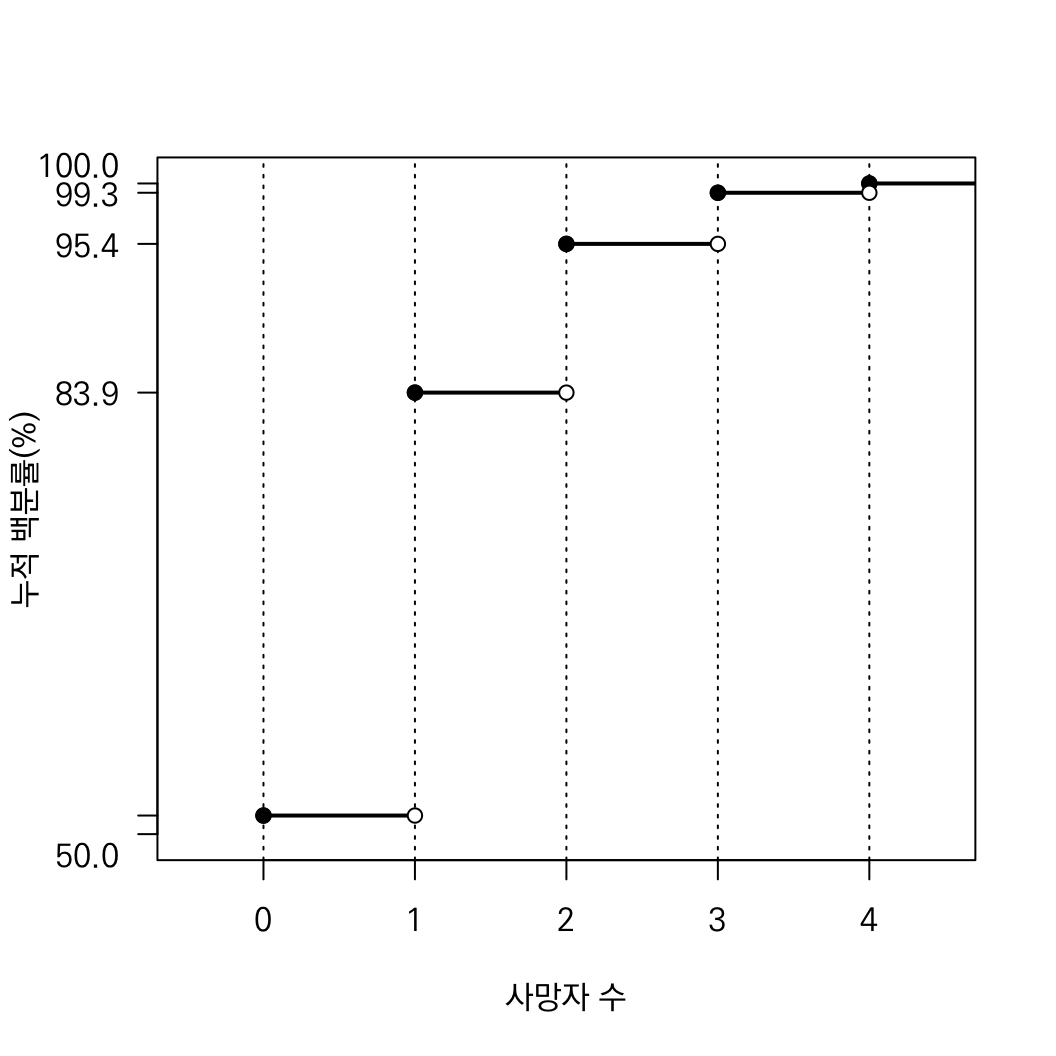
\includegraphics[width=0.75\linewidth]{JTBC_20150303_ggplot_v2_files/figure-latex/unnamed-chunk-5-1} \end{center}

\hypertarget{comments}{%
\subsection{Comments}\label{comments}}

Cheating Charts 를 학습하고 느낀 점을 간단히 기술합니다.

\end{document}
